\documentclass[tikz,border=6pt]{standalone}
\usepackage{amsmath,amssymb}
\usepackage{xcolor}
\definecolor{accent}{HTML}{A13D2C}
\definecolor{accent2}{HTML}{2B5F6B}
\definecolor{muted}{HTML}{5A564F}
\definecolor{panel}{HTML}{F8F6F0}
\definecolor{linecol}{HTML}{D8D2C4}
\definecolor{astroblue}{HTML}{1B4F72}
\definecolor{ink}{HTML}{1E1C1A}
\usetikzlibrary{calc,arrows.meta,decorations.markings}
\usepackage[T1]{fontenc}\usepackage{newpxtext,newpxmath}  % same fonts as the notes
\begin{document}
% Two ways to write mass conservation for a gas.
% (a) A box fixed in space. Gas crosses its walls; the mass inside changes by the net flow.
% (b) A blob that drifts with the gas. Nothing crosses its edge; its volume grows as the edge moves.
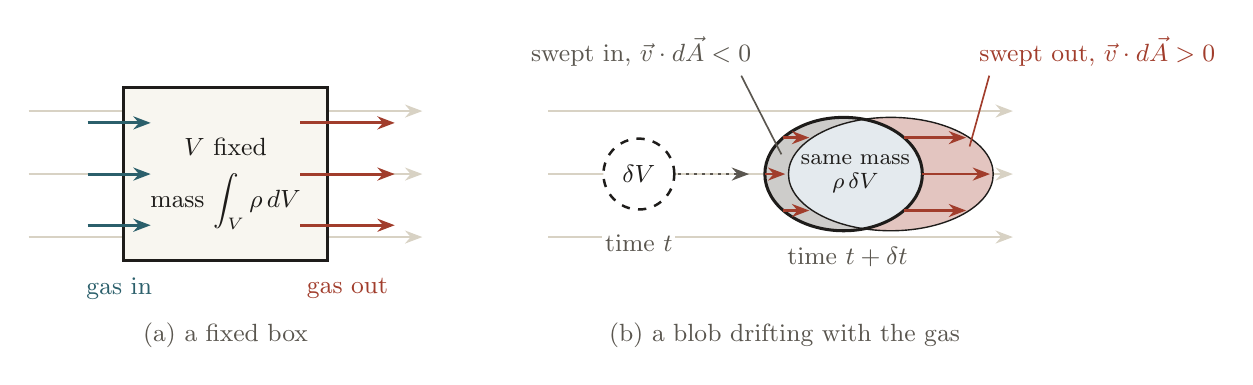
\begin{tikzpicture}[>={Stealth[length=2.2mm]}, font=\small]
  % ---------------- (a) fixed box ----------------
  \begin{scope}
    % background flow, speeding up to the right
    \foreach \y in {0.7,1.5,2.3}
      \draw[linecol, line width=0.7pt, ->] (-0.6,\y) -- (4.4,\y);
    \fill[panel] (0.6,0.4) rectangle (3.2,2.6);
    \draw[ink, line width=1.1pt] (0.6,0.4) rectangle (3.2,2.6);
    % gas crossing the walls: short arrows in on the left, longer arrows out on the right
    \foreach \y in {0.85,1.5,2.15}{
      \draw[accent2, line width=1.1pt, ->] (0.15,\y) -- (0.95,\y);
      \draw[accent, line width=1.1pt, ->] (2.85,\y) -- (4.05,\y);
    }
    \node[ink] at (1.9,1.85) {$V$ fixed};
    \node[ink] at (1.9,1.15) {mass $\displaystyle\int_V\rho\,dV$};
    \node[accent2, below, align=center] at (0.55,0.3) {gas in};
    \node[accent, below, align=center] at (3.45,0.3) {gas out};
    \node[muted] at (1.9,-0.55) {(a) a fixed box};
  \end{scope}
  % ---------------- (b) drifting blob ----------------
  % The gas moves right and speeds up to the right, so the right edge outruns the left edge.
  \begin{scope}[xshift=6.6cm]
    \foreach \y in {0.7,1.5,2.3}
      \draw[linecol, line width=0.7pt, ->] (-0.6,\y) -- (5.3,\y);
    % the blob at time t
    \draw[ink, dashed, line width=0.9pt, fill=white] (0.55,1.5) circle (0.45);
    \node[ink] at (0.55,1.5) {$\delta V$};
    \node[muted, fill=white, inner sep=1pt] at (0.55,0.62) {time $t$};
    \draw[muted, dotted, line width=0.9pt, ->] (1.05,1.5) -- (1.95,1.5);
    % the blob at t + dt (solid) and a moment later (thin): shifted right and wider
    \def\oldE{(3.15,1.5) ellipse (1.0 and 0.72)}
    \def\newE{(3.75,1.5) ellipse (1.3 and 0.72)}
    \fill[accent!30] \newE;
    \fill[muted!30] \oldE;
    \begin{scope}\clip \newE; \fill[astroblue!12] \oldE; \end{scope}
    \draw[ink, line width=1.1pt] \oldE;
    \draw[ink, line width=0.5pt] \newE;
    % every bit of the edge moves right with the gas, faster on the right
    \foreach \a in {0,40,140,180,220,320}{
      \pgfmathsetmacro{\L}{0.26+0.3*(1+cos(\a))}
      \draw[accent, line width=0.9pt, ->]
        ($(3.15,1.5)+({1.0*cos(\a)},{0.72*sin(\a)})$) -- ++(\L,0);
    }
    \node[ink, align=center, font=\footnotesize] at (3.3,1.5) {same mass\\[-1pt]$\rho\,\delta V$};
    \node[muted, fill=white, inner sep=1pt] at (3.2,0.45) {time $t+\delta t$};
    % labels for the two thin bands, away from the arrows
    \draw[accent, line width=0.6pt] (4.75,1.85) -- (5.0,2.75);
    \node[accent, anchor=south west, align=left] at (4.75,2.75) {swept out, $\vec v\cdot d\vec A>0$};
    \draw[muted, line width=0.6pt] (2.36,1.75) -- (1.85,2.75);
    \node[muted, anchor=south east, align=right] at (2.1,2.75) {swept in, $\vec v\cdot d\vec A<0$};
    \node[muted] at (2.4,-0.55) {(b) a blob drifting with the gas};
  \end{scope}
\end{tikzpicture}
\end{document}
